\chapter{Общие вопросы}

В этой главе приводятся основные понятия ML и DS. 


\section{Машинное обучение}

Машинное обучение (ML) - область искусственного интеллекта, изучающая самообучающиеся модели, то есть решаюшие поставленную задачу не по заранее запрограммированному алгоритму, а предварительно настраивая свое поведение согласно имеющимся данным. 

Обычно методы ML содержат свободные параметры, подбор которых наилучшим (в смысле имеющихся данных) образом и составляет процесс обучения алгоритма.


\section{Основные классы задач}


\section{Обнаружение аномалий}


\section{Контроль качества}

...оценка обобщающей способности...


\section{Недообучение}


\section{Переобучение}


\section{Регуляризация}


\section{Отбор признаков}


\section{Параметры алгоритма}


\section{Подбора метапараметров}


\section{Основные типы алгоритмов}


\section{Многоклассовая классификация}


\section{Дисбаланс классов}

...чем плохо... как бороться (over/undersampling/SMOTE)...


\section{Ансамбли алгоритмов}


\section{Метрики классификации}

Пусть некоторый алгоритм $a$ решает задачу бинарной классификации с классами $0$ (негативный) и $1$ (позитивный).
Тестирование алгоритма $a$ проводится на $n$ объектах, ответы $y$ на которых известны. Пусть $TP$ и $TN$ - числа правильно классифицированных позитивных и негативных объектов соответственно. Аналогично, $FP$ и $FN$ - числа неправильно классифицированных позитивных и негативных объектов соответственно.

О качестве алгоритма $a$ можно судить по матрице ошибок:
\begin{center}
\begin{tabular}{ c c c }
     & y=1 & y=0 \\ 
 a=1 & TP  & FP \\  
 a=0 & FN  & TN    
\end{tabular}
\end{center}

Для оценки качества работы алгоритмов бинарной классификации обычно используются описанные далее основные метрики.

\subsection{Accuracy}

Точность (accuracy) - отношение числа правильных ответов к общему количеству,

$$
accuracy = \frac{TP + TN}{n}.
$$

Проста в использовании и интерпретации, но плоха для несбалансированных выборок, и потому довольно редко используемая напрямую.

\subsection{Precision}

Точность (precision) - отношение числа правильно классифицированных позитивных объектов к общему количеству позитивно классифицированных,

$$
precision = \frac{TP}{TP + FP}.
$$

Чем ближе значение к 1, тем меньше ложных срабатываний (FP).

\subsection{Полнота (recall)}

Полнота (recall) - вычисляется как отношение

$$
recall = \frac{TP}{TP + FN}.
$$

Чем ближе значение к 1, тем меньше ложных пропусков (FN).

\subsection{F1-мера}

F1-мера - среднее гармоническое точности и полноты,

$$
F = \frac{2PR}{P + R}.
$$

F1-мера усредняет точность и полноту, является неплохом компромиссом между обеими метриками.

\subsection{F-мера}

Обобщенная F-мера вычисляется как

$$
F = (1+\beta^2)\frac{PR}{\beta^2P + R}.
$$

F-мера усредняет точность и полноту, является неплохом компромиссом между обеими метриками, имеет настраиваемый параметр $\beta$.

\subsection{ROC-AUC}

ROC-AUC - площадь под ROC кривой. 

Большинство алгоритмов бинарной классификации дают в качестве результата не просто $0$ или $1$, а некоторое число из отрезка $[0, 1]$. Окончательный ответ можно получить, задав некий порог $h$ - число, ниже которого ответ будет считаться принадлежащим классу $0$, а выше которого - классу $1$. 

Подбор наилучшего значения порога - отдельная задача, однако, есть метрики качества, позволяющие оценить алгоритм "в целом", без привязки к конкретному значению порога. ROC-AUC - одна из наиболее популярных метрик для такого рода оценки качества. 

Сама ROC кривая строится в координатах $TPR = TP/(TP + FN)$, $FPR = FP/(FP + TN)$ следующим образом:
\begin{enumerate}
    \item отрезки $[0, 1]$ по осям $TPR$ и $FPR$ разбиваются на $\#[y=0]$ и $\#[y=1]$ частей соответственно.
    \item пары реальных ответов $y_i$ упорядочиваются по убыванию соответствующих ответов алгоритма $a_i$
    \item проходя по получившемуся после сортировки массиву значений $y_i$, строим ROC кривую, начиная от начала координат и делая шаг вправо, если $y_i=0$ и вверх, если $y_i=1$
    \item важный момент: если рядом по порядку оказались несколько $a_i$ с одинаковыми значениями, то соответствующий им участок ROC кривой будет не ступенчатым, а прямолинейным (см. пример ниже).
\end{enumerate}


\textbf{Пример:}

\begin{tabular}{ c c }
    \raisebox{-\totalheight}{
    \begin{tabular}{|c|c|c|c|c|c|c|c|} 
        \hline
        y & 1 & 0 & 0 & 1 & 0 & 1 & 0 \\ 
        \hline
        a & 1.0 & 0.9 & 0.9 & 0.9 & 0.8 & 0.3 & 0.2 \\
        \hline
    \end{tabular}}
    & 
    \raisebox{-\totalheight}{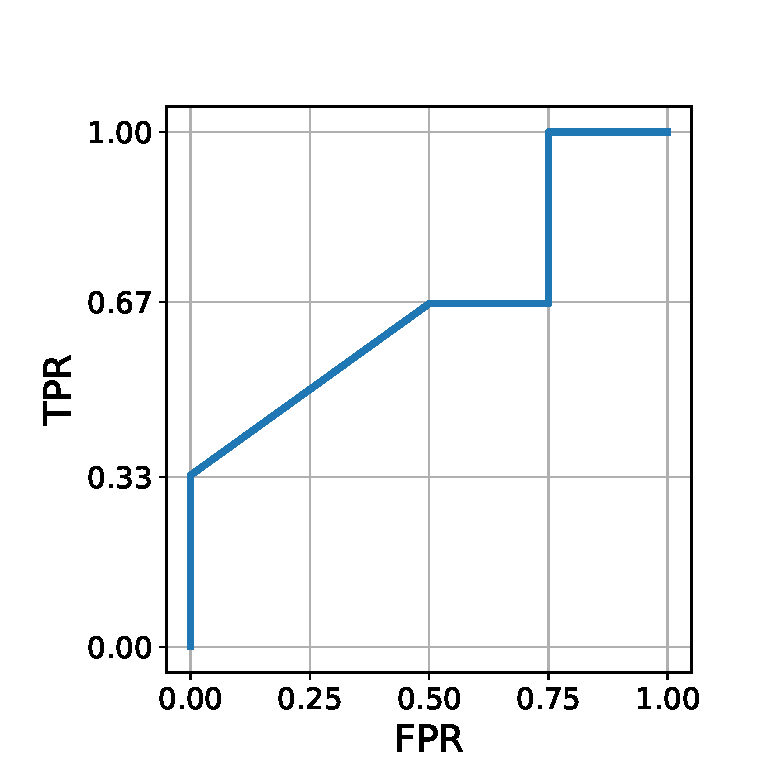
\includegraphics[scale=0.4]{images/roc-auc.eps}}
\end{tabular}

ROC-AUC более устойчива к дисбалансу классов, чем Accuracy, но не так хорошо, как PR-AUC. ROC-AUC также не учитывает уверенность алгоритма в своих предсказаниях (насколько близко распределены предсказания к $0$ и $1$).


\subsection{PR-AUC}

PR-AUC - площадь под PR кривой. Как и ROC-AUC, применяется для алгоритмов бинарной классификации, дающих не бинарный, а вероятностноподобный вывод и также оценивает алгоритм "в целом", без привязки к конкретному значению порога классификации.

Сама PR кривая строится в координатах $precision = TP/(TP + FP)$, $recall = TP/(TP + FN)$.

PR-AUC хороша для несбалансированных классов, так как учитывает $FP$ - число негативных объектов, неверно классифицированных как позитивные.


\section{Метрики многоклассовой классификации}


\section{ROC-AUC метрика}


\section{Индекс Джини}


\section{Метрики регрессии}


\section{Метрики кластеризации}


\section{Разложение ошибки алгоритма}


\section{Кривые валидации}


\section{Кривые обучения}


\section{Метрические методы}


\section{Метод ближайших соседей}


\section{Линейные методы}


\section{Линейная регрессия}


\section{Логистическая регрессия}

...отличие от линейной...


\section{SVM}


\section{Ядра и спрямляющие пространства}


\section{Решаюшие деревья}


\section{Случайный лес}

...отличие от беггинга над решающими деревьями...


\section{Градиентный бустинг}


\section{Байесовские методы}



